\documentclass[aspectratio=169,11pt, allowframebreak=0.9]{beamer}
\usepackage[czech]{babel}
%\usepackage[english]{babel}

\usepackage[default]{sourcesanspro}
\usepackage[T1]{fontenc}
\usepackage{marvosym}
\usepackage{csquotes}
\usepackage{graphicx}
\usetheme[sectionpage=none, progressbar=head]{metropolis}
\useoutertheme{infolines}
\setbeamersize{text margin left=1cm,text margin right=1cm}
\useinnertheme{rectangles}
\usecolortheme{beaver}
\title{Displeje}
\subtitle{Maturita z IVT}
\author{Jakub Šimek}
\institute[GEVO]{Gymnázium Evolution Jižní Město}
\date{\today}
\setcounter{tocdepth}{1}

\begin{document}
\normalfont
\section*{Titulní strana}
\begin{frame}
\titlepage
\end{frame}

\section*{Obsah}
\begin{frame}
\frametitle{Obsah}
\tableofcontents
\end{frame}
\section{Historické okénko}
\subsection{CRT}
\begin{frame}
\frametitle{Historické okénko: CRT displeje}
\begin{columns}
\column{0.6\textwidth}
\begin{itemize}
    \item \textbf{C}athode--\textbf{R}ay \textbf{T}ube
    \item Paprsek elektronů dopadá na sklo pokryté luminoforní (phosphor) vrstvou
    \item Vykreslování obrazu po řádcích
\end{itemize}
\column{0.5\textwidth}
\begin{figure}
    \centering
    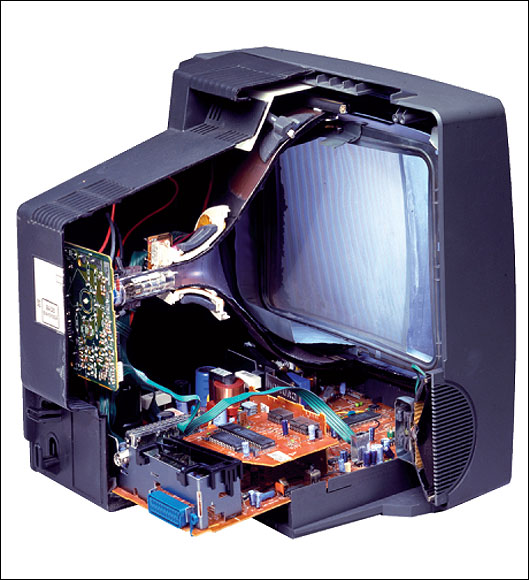
\includegraphics[width=0.7\textwidth]{crt.jpg}
    \caption{Průřez CRT displejem}
\end{figure}
\end{columns}
\end{frame}
\section{LCD}
\subsection{Obecné info}
\begin{frame}
\frametitle{LCD}
\begin{columns}
\column{0.6\textwidth}
\begin{itemize}
    \item \textbf{L}iquid \textbf{C}rystal \textbf{D}isplay
    \item Tekuté krystaly upravují polarizaci světla
    \item Orientace krystalů je řízena elektrickým polem
\end{itemize}
\column{0.5\textwidth}
\begin{figure}
    \centering
    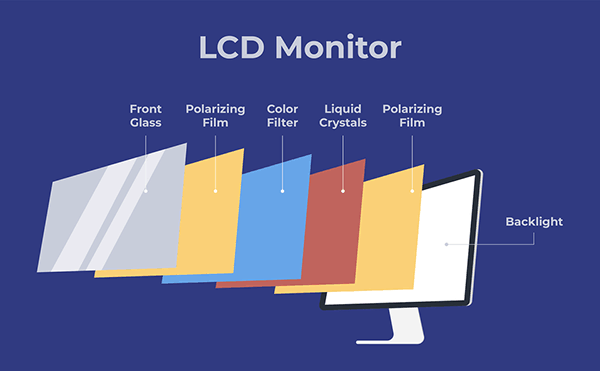
\includegraphics[width=1\textwidth]{lcd.png}
    \caption{Vrstvy LCD displeje}
\end{figure}
\end{columns}
\end{frame}
\subsection{TN}
\begin{frame}
\frametitle{Typy LCD: TN}
\begin{columns}
\column{0.6\textwidth}
\begin{itemize}
    \item \textbf{T}wisted \textbf{N}ematic displej
    \item Využívá nematické fáze tekutých krystalů
    \item Špatné pozorovací úhly
\end{itemize}
\column{0.5\textwidth}
\begin{figure}
    \centering
    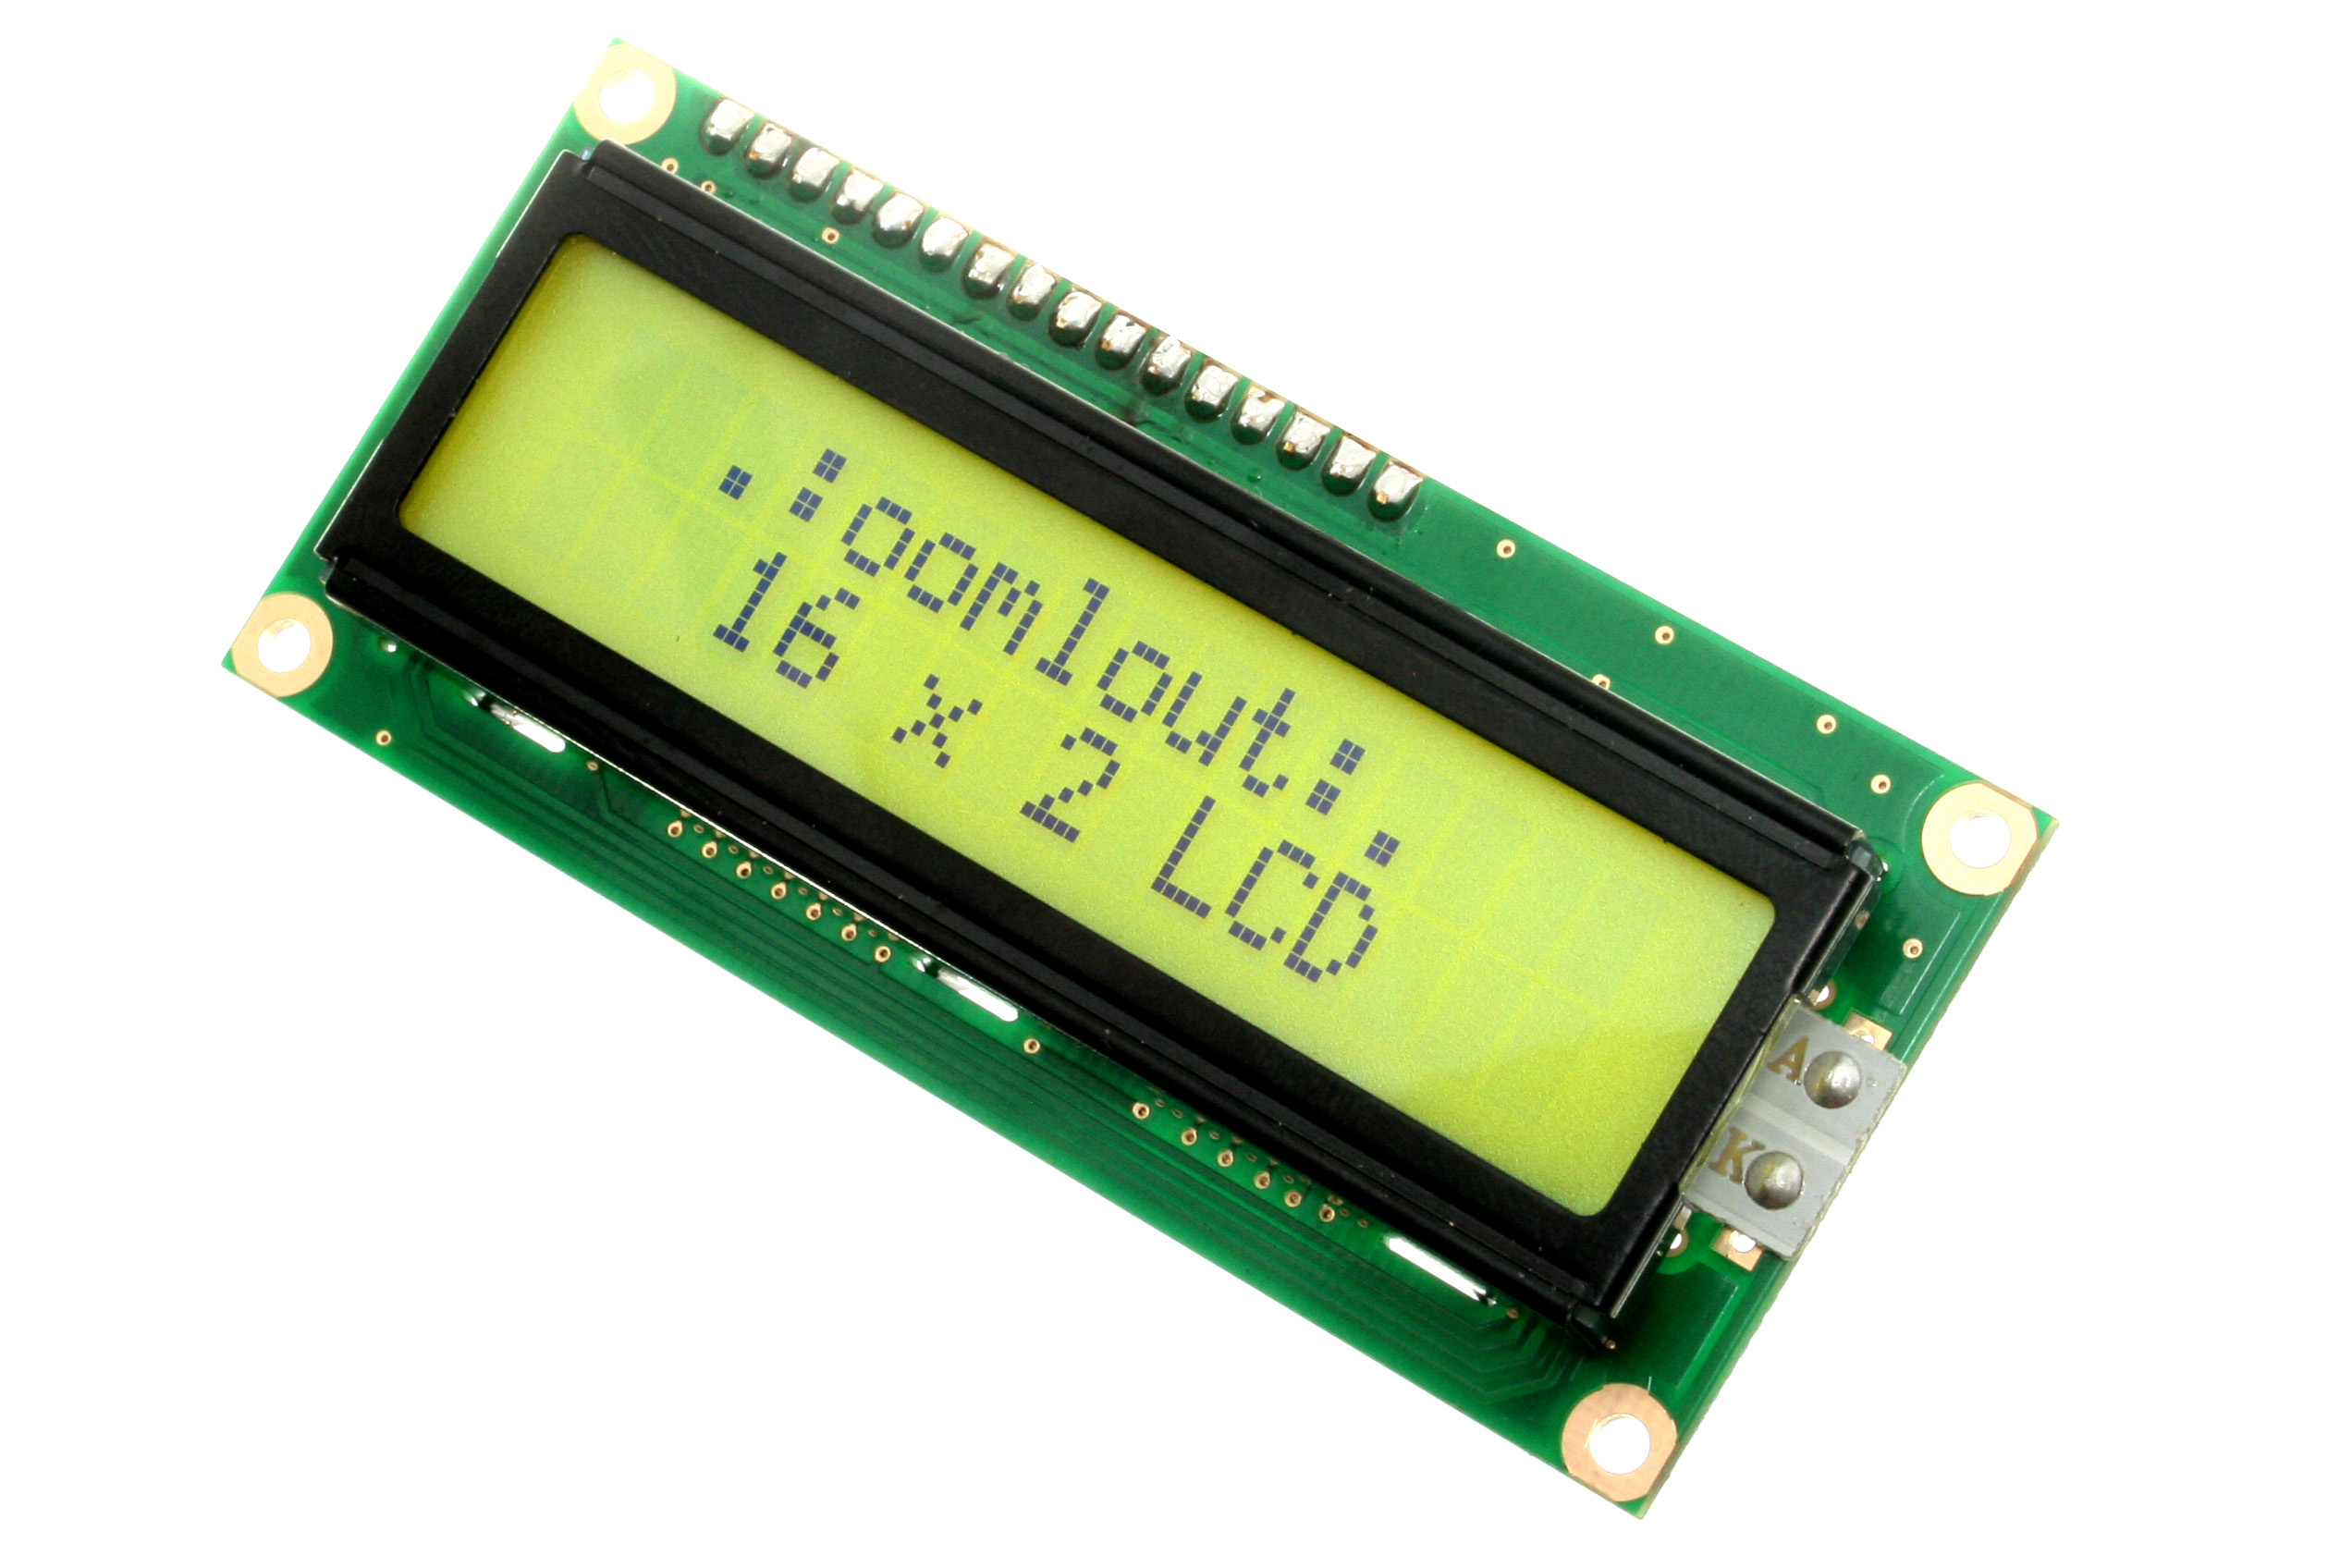
\includegraphics[width=1\textwidth]{dm.jpg}
    \caption{Dot-matrix TN displej}
\end{figure}
\end{columns}
\end{frame}
\begin{frame}
    \frametitle{Typy LCD: TN}
    \begin{columns}
    \column{0.5\textwidth}
    \begin{figure}
        \centering
        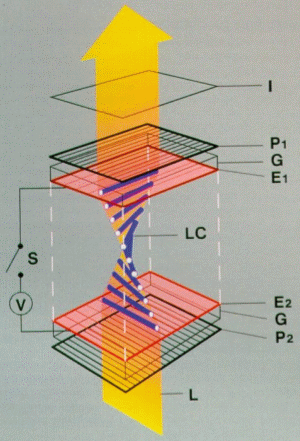
\includegraphics[width=0.5\textwidth]{tnOFF}
        \caption{Vypnutý TN displej}
    \end{figure}
    \column{0.5\textwidth}
    \begin{figure}
        \centering
        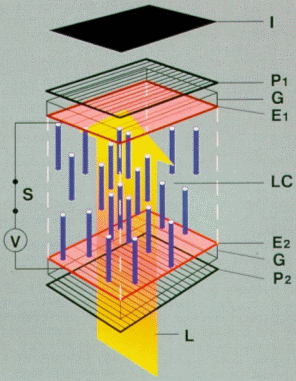
\includegraphics[width=0.5\textwidth]{tnON}
        \caption{Aktivní TN displej}
    \end{figure}
    \end{columns}
    \end{frame}
    \subsection{VA}
    \begin{frame}
    \frametitle{Typy LCD: VA}
    \begin{columns}
    \column{0.6\textwidth}
    \begin{itemize}
        \item \textbf{V}ertical \textbf{A}lignment
        \item Mnohem lepší zobrazení barev
        \item Lepší pozorovací úhly
    \end{itemize}
    \column{0.5\textwidth}
    \begin{figure}
        \centering
        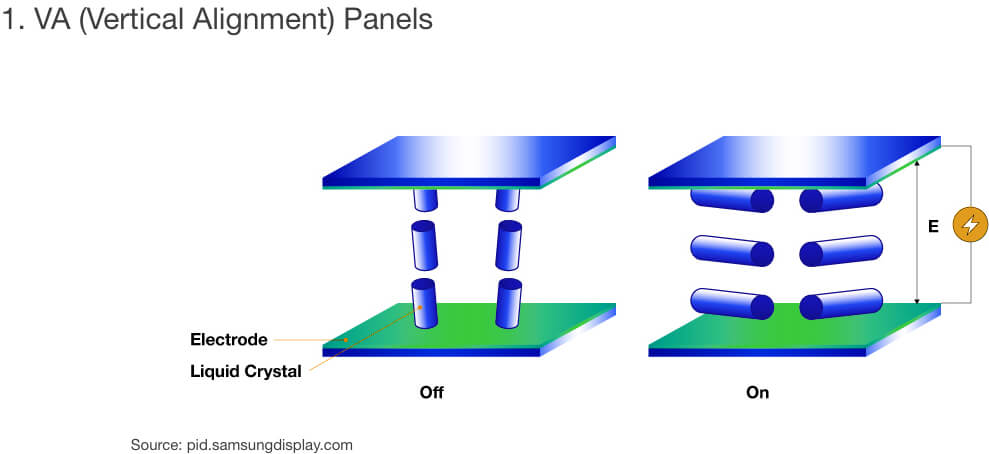
\includegraphics[width=1\textwidth]{va}
        \caption{Diagram VA panelu}
    \end{figure}
    \end{columns}
    \end{frame}
    \subsection{IPS}
    \begin{frame}
    \frametitle{Typy LCD: IPS}
    \begin{columns}
    \column{0.6\textwidth}
    \begin{itemize}
        \item \textbf{I}n \textbf{P}lane \textbf{S}witching
        \item Dobré zobrazení barev
        \item Dobré pozorovací úhly
    \end{itemize}
    \column{0.5\textwidth}
    \begin{figure}
        \centering
        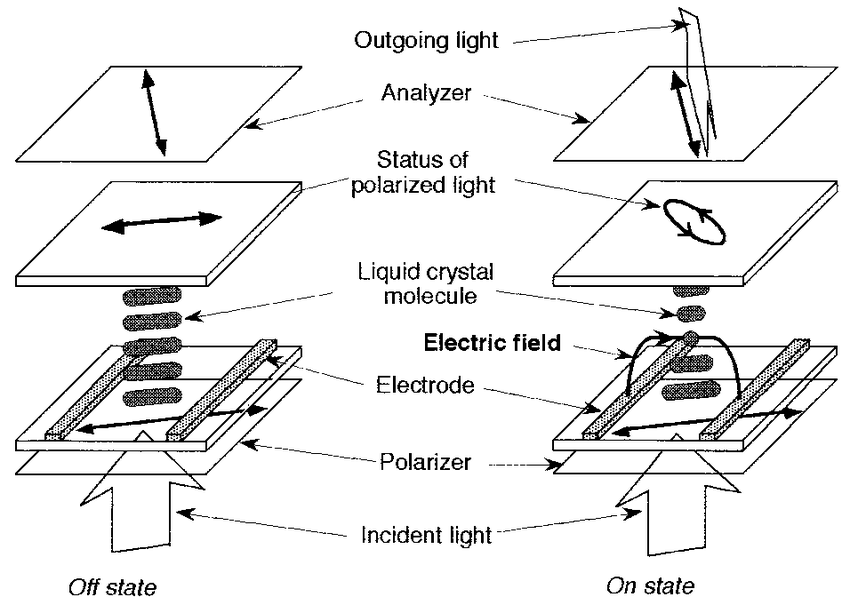
\includegraphics[width=1\textwidth]{ips}
        \caption{Diagram IPS panelu}
    \end{figure}
    \end{columns}
    \end{frame}
    \section{OLED}
    \subsection{}
    \begin{frame}
    \frametitle{OLED}
    \begin{columns}
    \column{0.6\textwidth}
    \begin{itemize}
        \item Každý pixel je samostatný světelný zdroj
        \item Výborný kontrast
        \item Výborné pozorovací úhly
    \end{itemize}
    \column{0.5\textwidth}
    \begin{figure}
        \centering
        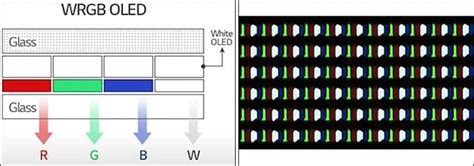
\includegraphics[width=1\textwidth]{oled}
        \caption{Diagram OLED panelu}
    \end{figure}
    \end{columns}
    \end{frame}
    \section{LED vs OLED}
    \begin{frame}
    \frametitle{LED vs OLED}
    \begin{columns}
    \column{0.6\textwidth}
    \begin{figure}
        \centering
        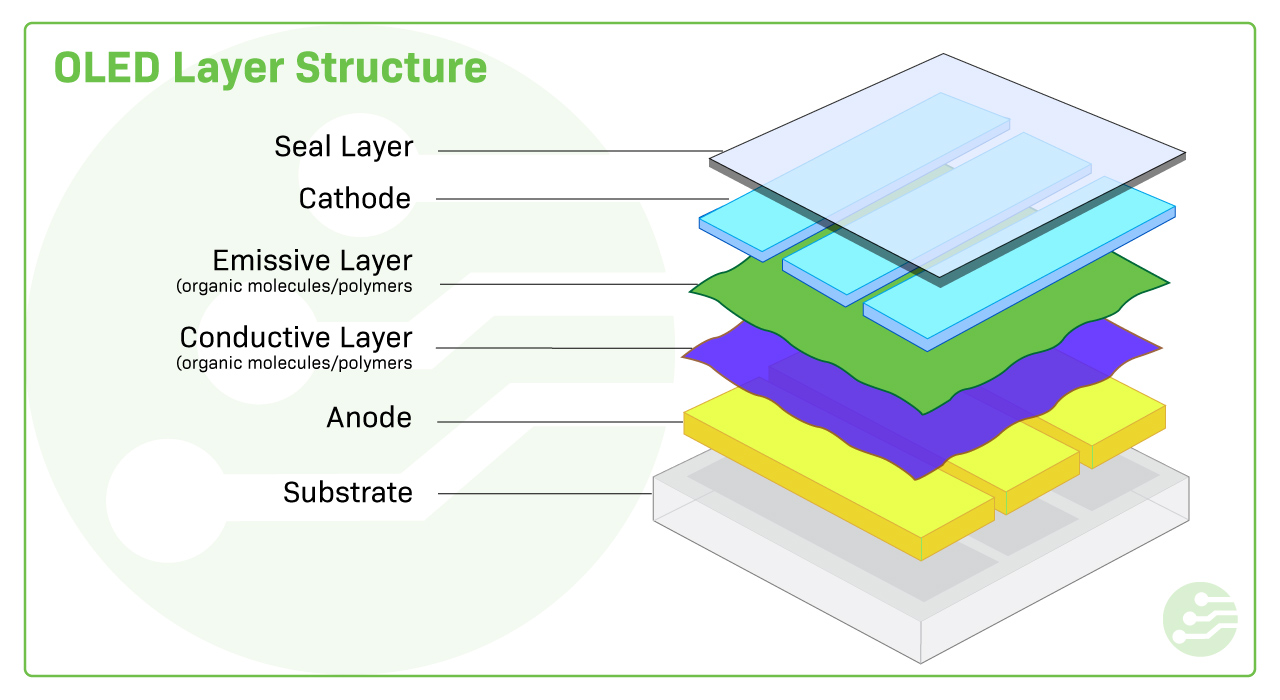
\includegraphics[width=1\textwidth]{oled2_.jpg}
       
    \end{figure}
    \column{0.5\textwidth}
    \begin{figure}
        \centering
        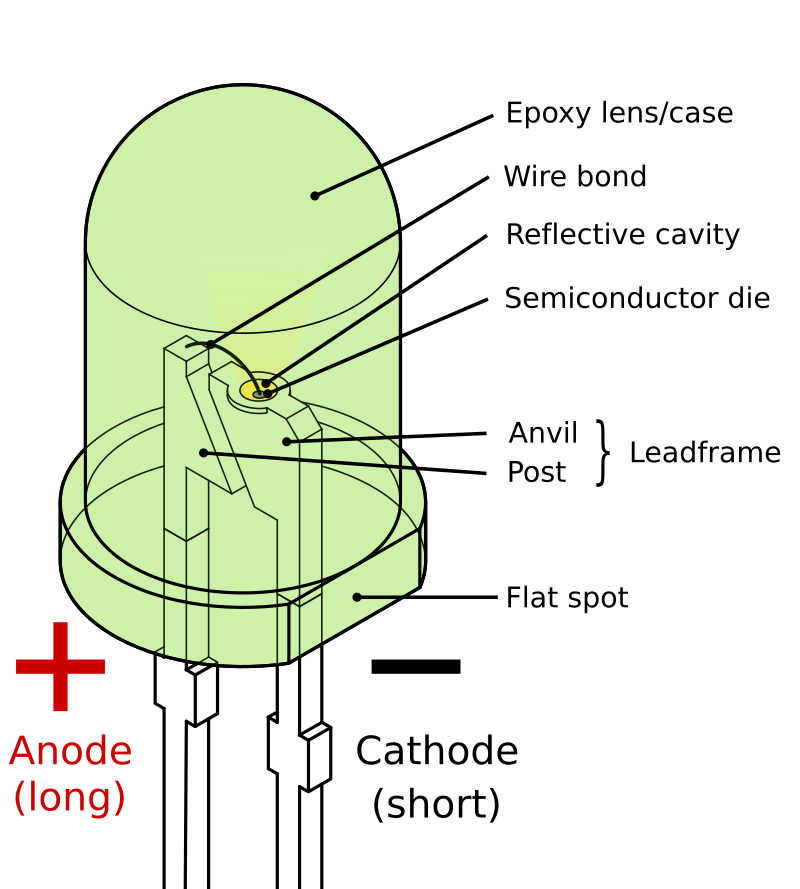
\includegraphics[width=0.8\textwidth]{led}
    
    \end{figure}
    \end{columns}
    \end{frame}
    \section{Další typy}
    \subsection{E Ink}
    \begin{frame}
    \frametitle{E Ink}
    \begin{columns}
    \column{0.6\textwidth}
    \begin{itemize}
        \item Elektroforetický displej
        \item Elektřina potřebná pouze pro změnu stavu
        \item Perfektní čitelnost na slunci
    \end{itemize}
    \column{0.5\textwidth}
    \begin{figure}
        \centering
        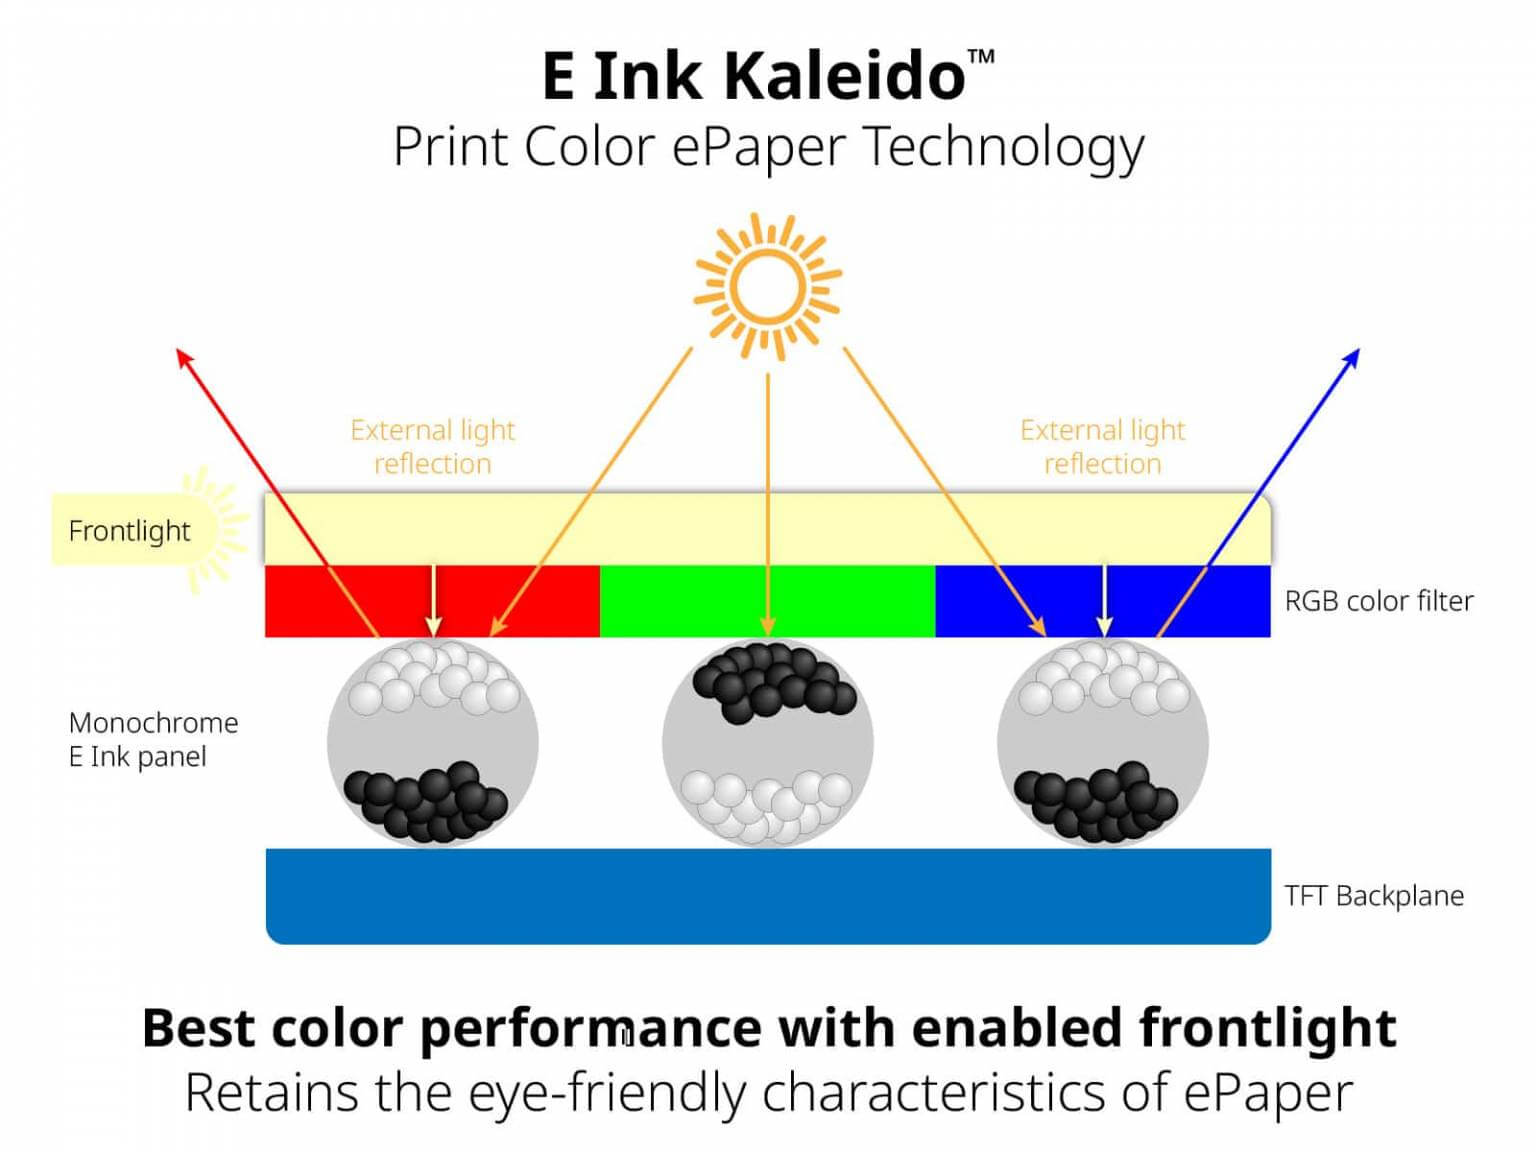
\includegraphics[width=1\textwidth]{eink}
        \caption{Diagram barevného E Ink panelu}
    \end{figure}
    \end{columns}
    \end{frame}
    \section{Parametry}
    \begin{frame}
        \frametitle{Co při nákupu?}
        \begin{itemize}
            \item Rozlišení
            \item Typ panelu
            \item Kontrast
            \item Odezva
            \item Refresh rate
        \end{itemize}
        
        \end{frame}
        \section{Projektory}
        \begin{frame}
            \frametitle{Projektory}
            \begin{itemize}
                \item Víceméně displej se supersilným podsvícením
                \item Čočka promítá obraz
                \item LCD
                \item DLP
            \end{itemize}
            
            \end{frame}
            \begin{frame}
                \frametitle{LED vs OLED}
                \begin{columns}
                \column{0.6\textwidth}
                \begin{figure}
                    \centering
                    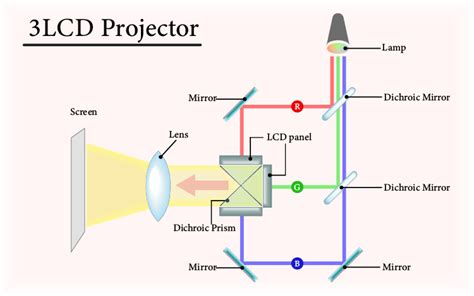
\includegraphics[width=1\textwidth]{lcdp}
                   
                \end{figure}
                \column{0.5\textwidth}
                \begin{figure}
                    \centering
                    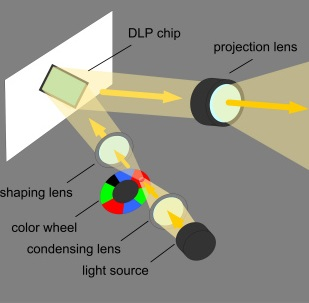
\includegraphics[width=0.8\textwidth]{dlp}
                
                \end{figure}
                \end{columns}
                \end{frame}
\section*{}
\begin{frame}[standout]
    \Huge
    Děkuji za pozornost
    \end{frame}


\end{document}